\chapter{Marco teórico}
\label{cap:marco}

\section{Marco teórico}

El siguiente capítulo describe los fundamentos teóricos necesarios para la comprensión del problema principal planteado en este trabajo, así como también la solución propuesta para este. 

\subsection{Radiointerferometría}

La radiointerferometría se basa en el teorema de Van Citter Zernicke  representado en la ecuación \Ref{eq:cittert-zernike}. Este relaciona directamente la función de visibilidad $V(u,v)$  y el mapa de misión de energia en radio-frecuencias ($I(x,y)$), es decir la imagen que se quiere obtener.  $(x,y)$ representan las coordenadas en radianes de la esfera celeste \citep{synthesis_taylor} y $(u,v)$ es el vector que para una medición use dos antenas en unidades de longitud de onda.

\begin{equation}
    I^{D}(x, y) = \int_{-\infty}^{\infty}\int_{-\infty}^{\infty}V(u, v)S(u,v)e^{-2\pi i (ux + vy)}dudv
    \label{eq:intensity}
\end{equation}

La captura de datos se realiza mediante puntos discretos en la Tierra (antenas) que capturan ondas electromagnéticas denominadas $E_i$. La correlación entre campos eléctricos recibidos por dos antenas ($E_i$ y $E_j$) se le denomina visibilidad y está representada por $V =<E_{i}E_{j}^{*}>$. Si esto se lleva al plano continuo ($u$,$v$) se obtiene lo mostrado en la ecuación \Ref{eq:intensity}.

Un problema es que la  imagen del cuerpo celeste no se puede obtener directamente debido a que el espacio de los datos no se encuentra regularmente muestreado (Figura \Ref{fig:uv_coverage}). Como paso intermedio se traspasan las muestras a una grilla regular lo que generar una gran fracción de celdas sin valor asignado. Esto conlleva a la estimación de $I(x,y)$ llamada imagen sucia, la cual asigna un valor 0 a las celdas sin valor y calcula la trasformada de Fourier. Encontrar una mejor imagen no está bien ya que este es un problema \textit{ill-posed} o mal puesto. Esto significa que desde un mismo conjunto de datos se puede obtener más de una imagen resultante \citep{levanda_art}.


\begin{figure}[!ht]
	\centering
	\captionsetup{justification=centering}
	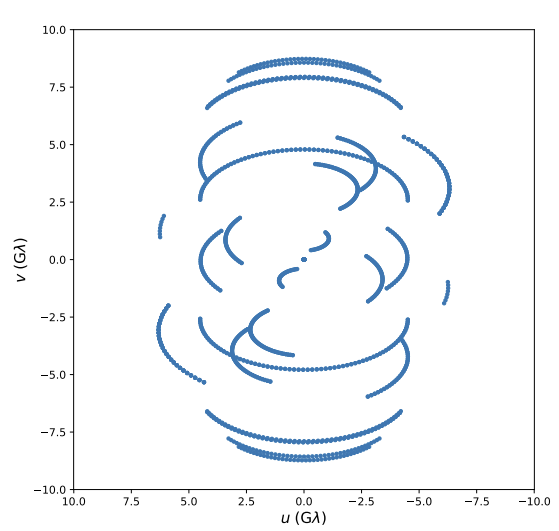
\includegraphics[scale=0.6]{images/uv_coverage.png}
	\caption[Cobertura en el plano $u-v$ para Sagitario A*.]{Cobertura en el plano $u-v$ para observacion de Sagitario A*. Fuente: \citep{Chael_2018}}
	\label{fig:uv_coverage}
\end{figure}

\subsection{Modelo de ruido}

El proceso de captura de datos siempre está sujeto a algún tipo de corrupción. En la radio-interferometría se capturan señales de radio provenientes de lugares lejanos en el espacio exterior, por lo que para llegar al planeta Tierra es necesario que esta señal atraviese distintos medios. Los detectores de señales instalados en cada antena deben ser refrigerados en helio líquido de forma de poder capturar las señales muy débiles \citep{Receivers} y por tanto sujetas al ruido térmico. Es así que los datos radio-interferómetros e imágenes resultantes del proceso de síntesis se encuentran corruptas por factores de ruido. 

Un modelo de ruido \citep{synthesis} utilizado en este trabajo es el presentado en la ecuación \Ref{eq:error2}, que muestra tanto un factor multiplicativo o ganancias y un factor aditivo que afecta a la visibilidad $V_{ij}$ capturada por par de antenas $i$ y $j$. 

\begin{equation}
    \tilde{V}_{ij}(t) = g_{i}(t)g^{*}_{j}(t)V_{ij}(t) + \epsilon_{ij}(t)
    \label{eq:error2}
\end{equation}

El factor multiplicativo o ganancias se produce por las distorsiones atmosféricas al momento de viajar la señal hacia la antena. Por otro lado, el factor aditivo se produce por el ruido térmico en el instrumento. A pesar de ser sometido a temperaturas muy bajas, esto no elimina completamente el ruido. 


\subsection{Síntesis de imágenes}
\label{subcap:sintesis}

La ecuación \Ref{eq:intensity} origina la ecuación \Ref{eq:intensity_conv} cuando se incluye la aproximación a imagen sucia. Donde $b_{0}$ se denomina \textit{beam} sintético y se define como $b_0 = \mathfrak{F}(S(u, v))$, donde $S$ es la función de muestreo. La función de muestreo es simplemente una suma de masas de Dirac ubicadas en las ubicaciones de las mediciones y con intensidad igual al peso.  Examinando la ecuación \Ref{eq:intensity_conv} se entiende que la imagen original se obtendría invirtiendo la operación de convolución . A este proceso se le denomina síntesis de imágenes \citep{synthesis}.  

\begin{equation}
\label{eq:intensity_conv}
    I^{D}(x,y) = I(x,y) **\ b_{0}(x,y)
\end{equation}

Existen diversos métodos para lograr esta deconvolución y así obtener la imagen, como por ejemplo CLEAN \citep{clean} o MEM \citep{sutton2006optimal}. Un método utilizado para la síntesis de imágenes es el utilizado en \citet{Chael_2018}, denominada Máxima verosimilitud regularizada. En esta se realiza la minimización de una función objetivo, donde a esta se le agregan funciones regularizadoras a la falta de información que existe del cuerpo o fenómeno detectado. La ecuación utilizada es la mostrada en \ref{eq:RML}.

\begin{equation}
 \label{eq:RML}
    J(I) = \sum_{data\ terms}\chi_{D}^{2}(I,d) - \sum_{regularizers} \beta_{R}S_{R}(I)
\end{equation}

donde $\chi_{D}^{2}$ es el modulo al cuadrado del residuo en un datos y $S_{R}$ son funciones regularizadoras. Cuyo objetivo es restringir el problema para llegar a una solución única, estas se especifican en \citet{Chael_2018}. Por otro lado, $\beta_{R}$ corresponden a los pesos que se le dan a las funciones regularizadoras correspondientemente. Una imagen reconstruida puede verse en la Figura \Ref{fig:m87}.

\begin{figure}[!ht]
	\centering
	\captionsetup{justification=centering}
	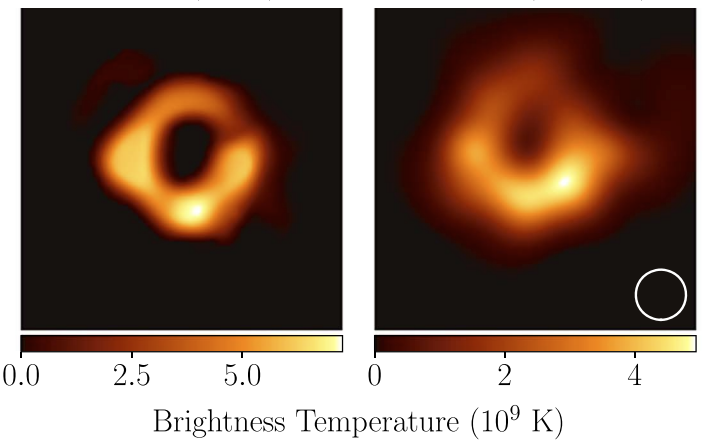
\includegraphics[scale=0.6]{images/Black_hole.png}
	\caption[Imagen reconstruida de agujero negro M87.]{Imagen reconstruida del agujero negro M87 mediante los métodos \textit{Regularized Maximum Likelihood} (RML) (izquierda) y CLEAN (derecha). Fuente: \citep{m87_image}}
	\label{fig:m87}
\end{figure}


\subsection{Datos radio-interferométricos}

Los datos capturados son guardados en un formato llamado \textit{measurement set} (MS) que son un conjunto de carpetas no relacionadas guardadas en disco. A continuación se describe los principales datos utilizados según \citep{kemball2000measurementset}.

\begin{itemize}
    \item \textbf{Visibilidad}: Corresponde al valor de la observación, es decir, el valor resultante de la ecuación \ref{eq:cittert-zernike}. Dicho valor pueden ser guardadas en tres columnas \texttt{DATA}, \texttt{MODEL} o \texttt{CORRECTED}. La columna \texttt{DATA} representa valores medidos en el interferometro o visibilidades observadas. La columna \texttt{CORRECTED} corresponde a valores corregidos por el proceso de {\it selfcalibration}. La columna \texttt{MODEL} son los valores estimados después de la síntesis de imágenes.
    \item \textbf{Pesos}: Es una estimación del valor inverso de la varianza para la visibilidad. Este valor es dado por el correlador. 
    \item \textbf{Antena}: Corresponde a las antenas asociadas a la observación. Estás están separadas en dos columnas denominadas \texttt{ANTENNA1} y \texttt{ANTENNA2}.
    \item \textbf{Tiempo}: Es el instante en el cúal se realizó la medición. 
    \item \textbf{UVW}: Es un vector 3D que une un par de antenas. 
    \item \textbf{Flag}: Indica que si el dato observado esta marcado como invalido, donde Verdadero indica inválido y Falso indica lo contrario. Este tiene las mismas dimensiones que las Visbilidades. 
    \item \textbf{\textit{Scan number}}: Número para identificar aquellas observaciones que se tomaron en el mismo instante. 
\end{itemize}

El software \texttt{casabrowser} \citep{casabrowser} permite acceder a los datos del MS de manera directa. Una tabla vista desde este programa se puede ver en la Figura \ref{fig:casabrowser}. 

\begin{figure}[!ht]
	\centering
	\captionsetup{justification=centering}
	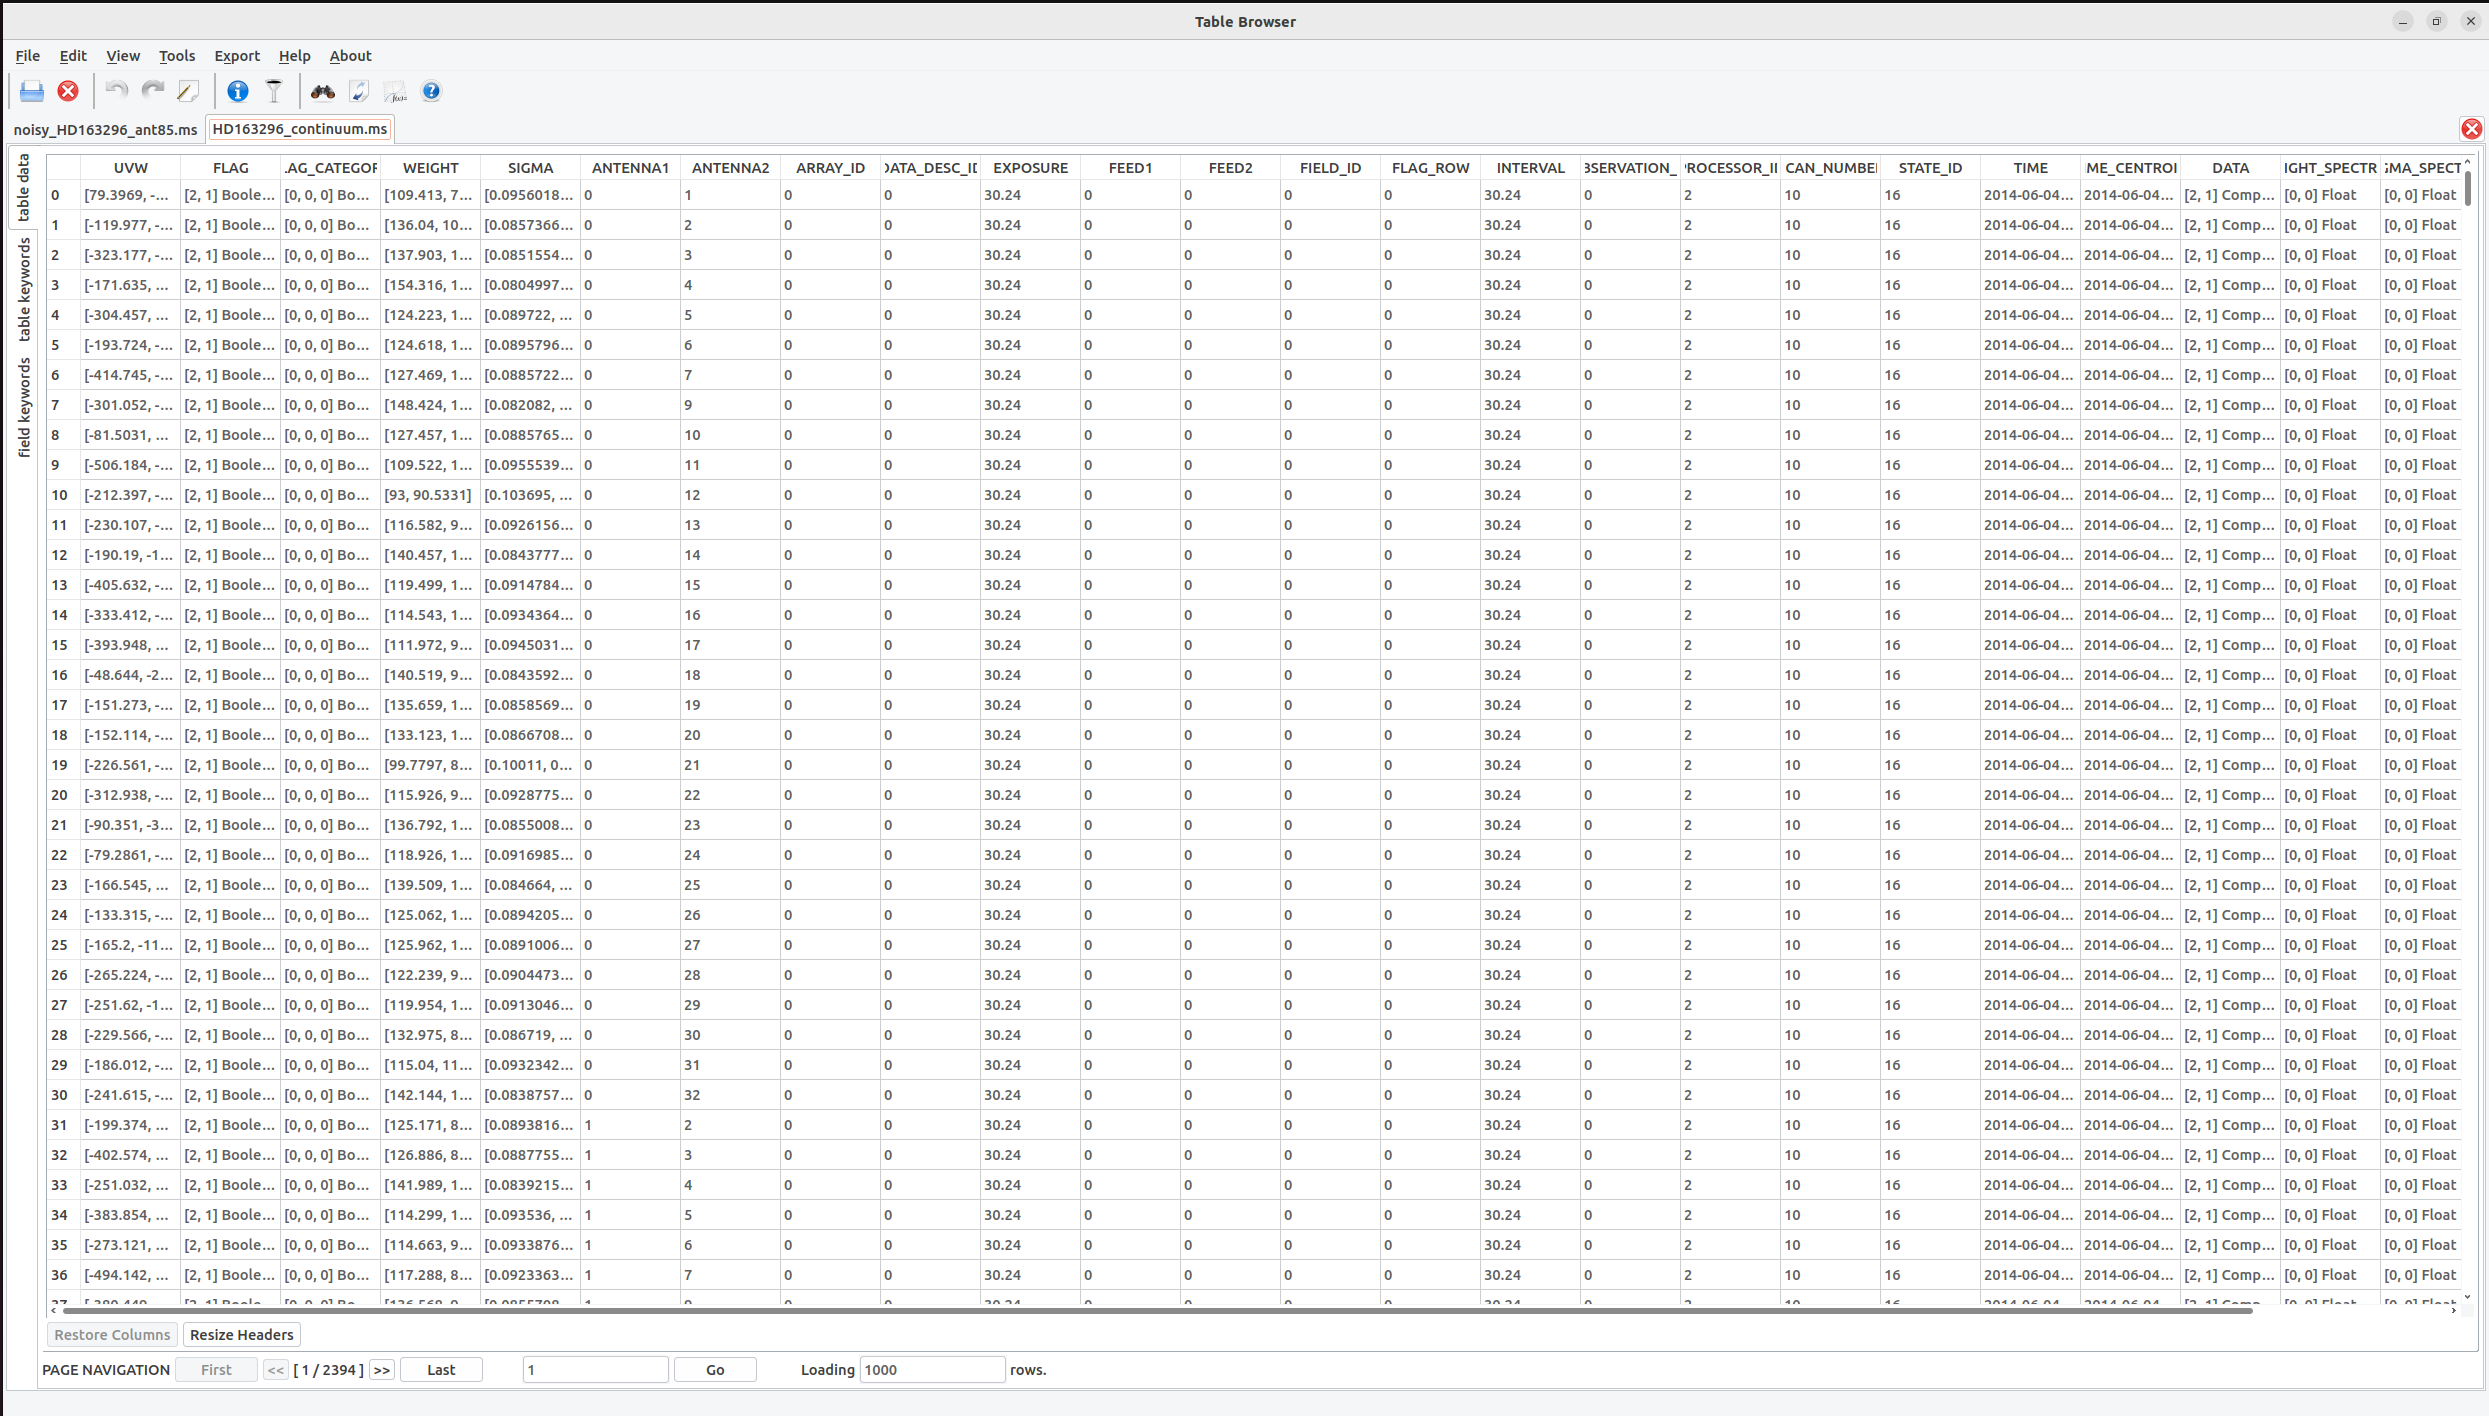
\includegraphics[scale=0.22]{images/casabrowser.png}
	\caption[Casabrowser]{Casabrowser. Fuente: Elaboración propia}
	\label{fig:casabrowser}
\end{figure}



\subsection{\textit{Self-calibration}}
\label{sec:selfcal}

Este procedimiento busca corregir las visibilidades observadas eliminando el ruido multiplicativo generado por turbulencias en la alta atmósfera. Se itera obteniendo un modelo de Imagen $I$ con el cual se obtienen visibilidades modelo con las cuales se estima las ganancias $g_i$ para corregir los datos. Para esto se deben estimar las ganancias $g_i$ y $g_j$ mediante la minimización de la ecuación \Ref{eq:min_self}.
%Este procedimiento busca obtener un modelo de distribución de intensidad $I$, en el cual su transformada de fourier $V$ al ser corregida por unos factores de ganancia se obtiene las visibilidades observadas sin el ruido que le afecta. Para esto se deben estimar las ganancias $g_i$ y $g_j$ mediante la minimización de la ecuación \Ref{eq:min_self}.

\begin{equation}
    S = \sum_{k}\sum_{\genfrac{}{}{0pt}{}{ij\hfill}{i \neq j\hfill}} w_{ij}(t_k) |\tilde{V}_{ij}(t_k) - g_i(t_k)g_{j}^*(t_k)\hat{V}_{ij}(t_k)|^2
    \label{eq:min_self}
\end{equation}

donde $w_{ij}(t_k)$ son pesos, $\tilde{V}_ij(t_k)$ las visibilidades modelo, $\hat{V}_{ij}(t_k)$ las visibilidades observadas y $t_{k}
$ es el intervalo de tiempo donde se obtienen las ganancias. Para corregir estos datos se debe seguir el algoritmo \ref{alg:optSelfCalibration} \citep{selfCalibration}. Cabe destacar que los pasos de este algoritmo se deben repetir hasta encontrar una imagen satisfactoria para el usuario. 

\begin{algorithm}[!ht]
	\caption{Algoritmo de \textit{self-calibration}}
	\label{alg:optSelfCalibration}
	\begin{algorithmic}[1]
	\REQUIRE $I$
	\ENSURE $V_{i,j,corr}$

        \STATE $V_{ij}, \tilde{V}_{ij} \gets reconstruction\_method(I)$

        \STATE $g_{i} , g_{j}^{*} \gets Min( \sum |V_{ij} - g_{i}g_{j}^{*}\tilde{V}_{ij}|^2)$  

        \STATE $V_{i,j,corr} \gets \frac{\tilde{V}_{ij}}{g_{i}g_{j}^{*}}$

        \Return $V_{i,j,corr}$
	
	\end{algorithmic}
\end{algorithm}

\begin{comment}
\begin{enumerate}
    \item Calcular un modelo de datos basado en una imagen modelo ($\tilde{V}=V^{m}(I)$).
    \item Minimizar la ecuación \ref{eq:self-calibration}
    \begin{equation}
        \sum |V_{ij} - g_{i}g_{j}^{*}\tilde{V}_{ij}|^2
        \label{eq:self-calibration}
    \end{equation}
    \item Aplicar los $g_{i}$ encontrados según la ecuación \ref{eq:self-calibration-2}
    \begin{equation}
        V_{i,j,corr} = \frac{\tilde{V}_{ij}}{g_{i}g_{j}^{*}}
        \label{eq:self-calibration-2}
    \end{equation}
    \item Analizar resultado obtenido, en caso de no ser satisfactorio volver a paso 1. 
\end{enumerate}
\end{comment}


\subsection{\textit{Bispectrum}}
\label{subsec:bispectrum}

El interferómetro comúnmente captura datos a través de pares de antenas, denominado visibilidad $V_{ij}$. Sin embargo, si se multiplican los valores de visibilidades de tríos de antenas se consiguen datos que no son afectados en su fase \citep{1958MNRAS.118..276J}. A este dato se le conoce como \textit{closure phase} o \textit{bispectrum} y se le representa mediante $V_{ijk}$ (ecuación \Ref{eq:bispectrum}), siendo $k$ la tercera antena incorporada. De esta manera, en un arreglo de $N$ elementos, se tiene $\frac{1}{2}N(N-1) - (N-1)$ \textit{closure phases}.

\begin{equation}
    V_{ijk} = V_{ij}V_{jk}V_{ki}
    \label{eq:bispectrum}
\end{equation}


Lo anterior puede ser demostrado si se toma la fase de la ecuación \Ref{eq:error3}, se obtiene lo mostrado en la ecuación \Ref{eq:phase}. Una derivación mas detallada de esta ecuación se encuentra en el Anexo \Ref{finales:anexo1}.

\begin{equation}
    \tilde{V}_{ij}(t) = g_{i}(t)g^{*}_{j}(t)V_{ij}(t) + \epsilon_{ij}(t)
    \label{eq:error3}
\end{equation}

\begin{equation}
\label{eq:phase}
    \tilde{\phi}_{ij}(t) = \phi_{ij}(t) + \theta_{i}(t) - \theta_{j}(t) + ruido.
\end{equation}

Donde $\theta_{i}(t) = arg g_{i}(t)$. Si se supone un conjunto de tres antenas $i$, $j$ y $k$, junto con la ecuación \Ref{eq:phase} mostrada anteriormente, se obtiene lo mostrado en la ecuación \Ref{eq:noGain}, donde $\tilde{C}_{ijk}(t)$ es la \textit{closure phase} observado. 

\begin{equation} \label{eq:noGain}
\begin{split}
\tilde{C}_{ijk}(t) & = \tilde{\phi_{ij}(t)} + \tilde{\phi_{jk}(t)} + \tilde{\phi_{ki}(t)}\\
 & = \phi_{ij}(t) + \phi_{jk}(t) + \phi_{ki}(t) + ruido \\
 & = C_{ijk}(t) + ruido
\end{split}
\end{equation}

De la ecuación \Ref{eq:noGain} se desprende que el \textit{bispectrum} no es afectado por el factor de fase en la ecuación de ruido.

El numero total de combinaciones que se pueden dar entre tres antenas esta dada por la ecuación $\binom{N}{3}$ donde $N$ son la cantidad de antenas, esto puede dar una gran cantidad de combinaciones conllevando a una gran carga de trabajo. Para fines de reducir la cantidad de datos se define una antena de referencia para trabajar solo con los tríos de antenas que incluyan a esta antena de referencia. Esto logra que la cantidad posible de combinaciones este dada por la ecuación \ref{eq:comb}, conllevando una disminución en la cantidad de combinaciones y también en la carga de trabajo \citep{Chael_2018}. 

\begin{equation}
\label{eq:comb}
    \binom{N-1}{2} = \frac{(N - 1)(N - 2)}{2}
\end{equation}


\subsection{Métricas de comparación}

\subsubsection{\textit{Peak signal-to-noise ratio(PSNR)}}

Este estimador es utilizado para medir la calidad de la imagen reconstruida, donde se compara el valor máximo de la señal y el valor promedio del ruido que la afecta. Para el contexto de síntesis de imágenes, se entiende como señal a la imagen que se quiere restaurar y al ruido como la diferencia entre la reconstrucción y la imagen original. La fórmula para calcular este estimador está dada por la ecuación \Ref{eq:psnr} \citep{LiberonaTesis}.

\begin{equation}
\label{eq:psnr}
    PSNR = 20 \cdot \log_{10}(\frac{MAX_{I}}{\sqrt{MSE}})
\end{equation}

Si el PSNR aumenta, el resultado se considera mejor pues indica que el brillo del objeto es mayor en comparación al ruido de fondo. Por el contrario, si los valores se parecen, significa que el objeto no se distingue correctamente debido a que se pierde en el ruido de fondo \citep{CeledonTesis}. 


\subsubsection{Raíz del error cuadrático medio (NRMSE)}
\label{sec:nrmse}

El NRMSE por su nombre en inglés \textit{simple normalized root-mean-square error} es una métrica que permite la comparación entre imágenes. Esta es una métrica punto a punto que permite evaluar las imágenes basadas en similitudes píxel a píxel. Por lo que si se tiene una imagen $A$ y una $B$ con $M$ píxeles, el NRMSE de $A$ relativo a $B$ se puede apreciar en la ecuación \Ref{eq:nrmse} \citep{Chael_2018}.

\begin{equation}
    \label{eq:nrmse}
    NRMSE(A,B) = \frac{\sqrt{\sum_{i=1}^{M}(A_i - B_i)^2}}{\sqrt{\sum_{i=1}^M B_{i}^2}}
\end{equation}


\begin{comment}
\subsection{Programación en GPU}

La programación en CPU y GPU tienen su principal diferencia en que la primera tiene un enfoque a ejecutar una secuencia de operaciones (\textit{thread}) lo mas rápido posible y además puede ejecutar una docena de estas en paralelo. En cambio, la tecnología GPU tiene un enfoque para ejecutar cientos de \textit{threads} en paralelo, permitiendo así un tiempo de ejecución menor \citep{nvidiaCuda}. 

Cada función que es llamada desde la CPU (\textit{host}) para ser ejecutada en GPU (\textit{device}) se denomina kernel. Este es ejecutado por $K$ diferentes \textit{CUDA Core}, las cuales son la unidad básica de procesamiento \citep{nvidia_cuda}. Para la ejecución del \textit{kernel}, las hebras son agrupadas en bloques (\textit{blocks}) y estos son agrupados en una grilla (\textit{grid}) que puede tener desde una hasta tres dimensiones \citep{nvidia_programming}. Un ejemplo de grilla y su organización de bloques puede ser vista en la Figura \Ref{fig:grid_nvidia}.

Los bloques son enviados a un \textit{streaming multiprocessor (SM)} para la ejecución del kernel. El multiprocesador crea, maneja, gestiona y ejecuta las hebras en grupos de 32 llamados \textit{warps}. Cada hebra que forma parte del \textit{warp} comienza en la misma dirección del programa, pero cada uno tiene su propio contador de dirección por lo que cada una puede ejecutarse de manera independiente. Además, cada warp tiene su propia memoria compartida \citep{nvidia_hardware}. 

Cuando una grilla junto a sus bloques han sido organizados, se puede identificar una hebra tanto de manera global como local. Para lograr esto existen diversos métodos que se listan a continuación \citep{nvidia_grid}. 

\begin{itemize}
    \item \textit{blockIdx.x, blockIdx.y, blockIdx.z:} identificador del bloque en una grilla para cada una de sus dimensiones. 
    \item \textit{gridDim.x, gridDim.y, gridDim.z:} cantidad de bloques en la dimensión correspondiente de la grilla. 
    \item \textit{threadIDx.x, threadIDx.y, threadIDx.z:} identificador de una hebra dentro de un bloque para cada una de sus dimensiones. 
    \item \textit{blockDim.x, blockDim.y, blockDim.z:} cantidad de hebras en la dimensión correspondiente del bloque. 
    \item \textit{blockDim.x\ blockIdx.x + threadIdx.x:} ID global de la hebra en la dimensión x.  
\end{itemize}

\begin{figure}[!ht]
	\centering
	\captionsetup{justification=centering}
	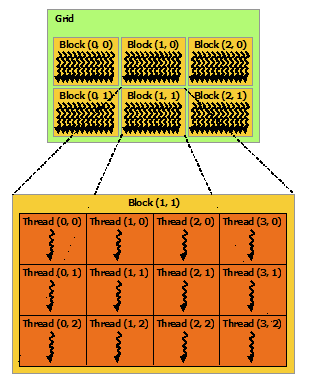
\includegraphics[scale=0.6]{images/grid_nvidia.png}
	\caption[Organización de grilla GPU.]{Organización de grilla GPU. Fuente: \citep{nvidia_programming}}
	\label{fig:grid_nvidia}
\end{figure}
\end{comment}

\subsection{Programación orientada a objetos (POO)}

La idea principal de la programación orientada a objetos (POO) es programar en términos de objetos y clases de tal manera de representar la vida real (Figura \Ref{fig:poo_image}). Este ultimo se entiende como un modelo o plano para poder crear objetos, permitiendo así guardar datos y funcionalidades. En cambio, los objetos son instancias de una clase, las cuales tienen métodos y atributos que intentan simular un objeto de la vida real. Algunos conceptos a tener en consideración son los siguientes \citep{tatachar2021object}. 

\begin{itemize}
    \item \textbf{Atributos:} Valores que son contenidos dentro de la clase. Estos pueden ser atributos de clases que son aquellos que se comparten entre todos los objetos, o pueden ser atributos de instancia, que son aquellos asociados a un objeto. 
    \item \textbf{Métodos:} Son funciones asociadas al objeto que permiten el comportamiento de este.
    \item \textbf{Herencia:} Característica que permite a una clase heredar los atributos y métodos de una clase padre o superior. 
    \item \textbf{Polimorfismo:} Permite que una acción sea ejecutada de distintas maneras. Por ejemplo, la operación suma en Python tiene diferentes resultados cuando se realiza con enteros o con \textit{strings}.
\end{itemize}

\begin{figure}[!ht]
	\centering
	\captionsetup{justification=centering}
	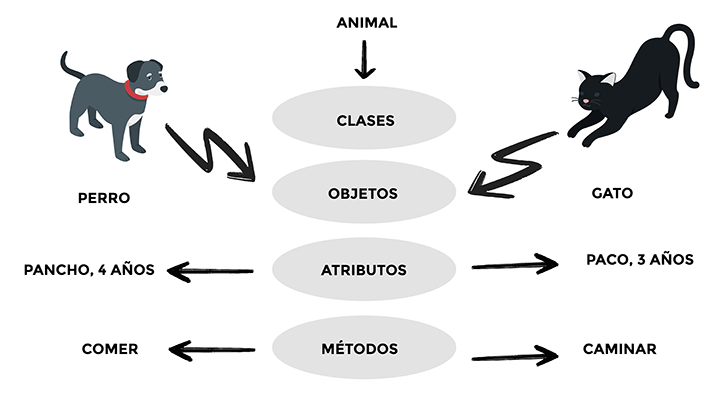
\includegraphics[scale=0.6]{images/POO.png}
	\caption[Ejemplo de abstracción del mundo real a POO.]{Ejemplo de abstracción del mundo real a POO. Fuente: \citep{poo_image}}
	\label{fig:poo_image}
\end{figure}

\subsection{Patrones de diseño}
\label{subsec:patrones}

Una definición bien utilizada para estos puede ser encontrada en  \cite{gamma2002patrones}, donde se menciona que los patrones de diseños son descripciones de objetos y clases interconectados que se adaptan para solucionar problemas de diseño generales en contextos específicos. Para esto un patrón de diseño debe contar con lo siguiente: 

\begin{itemize}
    \item \textbf{Nombre de patrón}: Sirve para describir el problema, la solución y la consecuencia en una o dos palabras. De esta manera se amplia el vocabulario de los patrones, permitiendo una mejor comprensión y comunicación de este. 
    \item \textbf{Problema}: Cuando aplicar el patrón de diseño. Este puede ser tanto de problemas de diseño específicos o describir estructuras de clases u objetos que son sintomáticas de un diseño inflexible. Además estos pueden incluir condiciones que especifiquen si se puede ocupar o no el patrón de diseño. 
    \item \textbf{Solución}: Son los elementos que contribuyen al diseño, sus relaciones, responsabilidades y colaboraciones. Es una plantilla abstracta que se adapta a diferentes situaciones, ofreciendo una solución general a un problema de diseño. 
    \item \textbf{Consecuencia}: Este es el resultado y compensación de aplicar el patrón de diseño, y son fundamentales para realizar un análisis para así comprender los costos y beneficios de su implementación. Entre las consecuencias que puede traer un patrón de diseño se considera su impacto en la flexibilidad, extensibilidad o portabilidad de un sistema.
\end{itemize}

Entre los patrones de diseño existentes en la realidad se puede encontrar el \textit{Decorator}, que permite añadir nuevas funcionalidades a un objeto dinámicamente a través de encapsular el objeto con otro objeto. Un diagrama de objetos que representa esta implementación es el mostrado en la figura \ref{fig:gamma2002patrones} y una implementación sencilla de código Python puede ser encontrada en el apéndice \ref{finales:apendice2}.

\begin{figure}[!ht]
	\centering
	\captionsetup{justification=centering}
	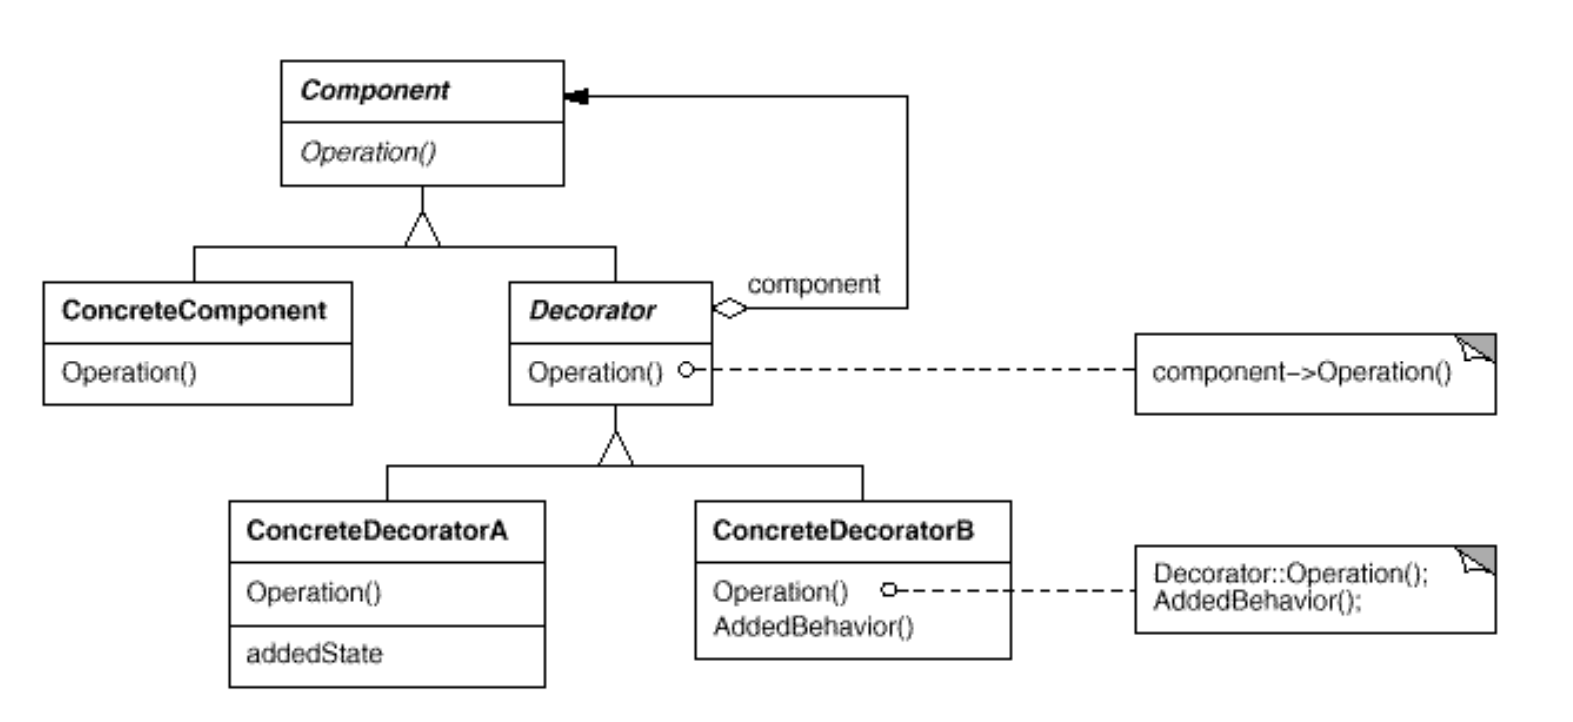
\includegraphics[scale=0.3]{images/decorator.png}
	\caption[Patrón de diseño Decorator.]{Patrón de diseño Decorator. Fuente: \citep{gamma2002patrones}}
	\label{fig:gamma2002patrones}
\end{figure}

Entre las ventajas que se encuentran del patrón de diseño \textit{Decorator} son no influir en las funcionalidades de otros objetos de la misma clase, así como también permite ejecutar funcionalidades del componente mismo, por lo que se pueden realizar acciones antes o después de esta ejecución. Además permite evitar la creación de clases cargadas de funcionalidades en lo alto de la jerarquía debido a que se puede crear una clase simple y agregar funcionalidades de manera incremental a través de decoradores. 

Sin embargo, las desventajas de este son que el componente y el decorador no son iguales desde el punto de vista de la identidad del objeto, debido a que el decorador solamente es un envoltorio. Por otro lado, aumentan la complejidad del código ya que existen muchos objetos pequeños que se parecen pero la manera en la que están interconectados difieren. 


\subsection{Pyralysis}
\label{subsec:pyralysis}

\textit{Python Radio Astronomy Analysis and Image Synthesis} (\textit{Pyralysis}) es un framework desarrollado en el lenguaje de programación Python junto a el paradigma de orientación a objetos (POO). Este tiene como objetivo facilitar el trabajo de los investigadores al tratar con datos radio-interferometricos automatizando procesos. Este framework actualmente se encuentra en desarrollo, pero mayor información puede ser encontrada en su repositorio de Gitlab \citep{winNT}.

\subsection{Computación paralela}

La computación paralela permite ejecutar varias instrucciones al mismo tiempo \citep{parallel}, por lo que para aprovechar esto en la programación existen diversas herramientas como es el caso de Dask, la cual es una librería para computo paralelo en Python \citep{Dask_general}. Dentro de Dask existe una colección conocida como \verb|Dask.array|, la cual es una copia de la interfaz de Numpy y permite separar grandes arreglos de datos en unos mas pequeños denominados bloques y que se ordenan a través de una grilla \citep{Dask_array}.  

\begin{figure}[!ht]
	\centering
	\captionsetup{justification=centering}
	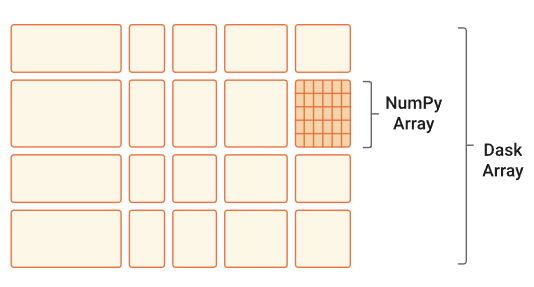
\includegraphics[scale=0.6]{images/dask_array.png}
	\caption[Organización de Dask array.]{Organización de Dask array. Fuente: \citep{Dask_array}}
	\label{fig:dask_array}
\end{figure}

Estos grandes arreglos son divididos en \textit{chunks} para así lograr el procesamiento paralelo y distribuido, por lo que se debe escoger un buen valor para estos ya que puede afectar de manera negativa el rendimiento en caso de una mala elección \citep{Dask_chunks}. Los \textit{chunks} tiene un tamaño firme y uniforme, el cual debe ser de un tamaño lo suficientemente pequeño para caber en memoria pero lo suficientemente grandes para que las tareas se ejecuten hasta en 1ms, normalmente estos van desde 10MB hasta 1GB. 

\begin{figure}
 \centering
  \subfloat[Arreglo Original]{
   \label{fig:chunk_or}
    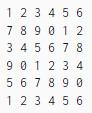
\includegraphics[width=0.2\textwidth]{images/chunk_or.png}}
  \subfloat[Arreglo con \textit{chunks} igual a 3]{
   \label{fig:chunk_3}
    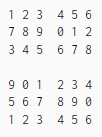
\includegraphics[width=0.19\textwidth]{images/chunk_3.png}}
    \subfloat[Arreglo con \textit{chunks} igual a (3,2)]{
   \label{fig:chunk_32}
    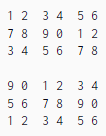
\includegraphics[width=0.2\textwidth]{images/chunk_32.png}}
 \caption[Arreglo dividido por chunks]{Arreglo dividido por \textit{chunks}. Fuente: \citep{Dask_chunks}.}
 \label{fig:chunks}
\end{figure}


Para lograr una computación paralela \verb|Dask.array| trabaja con grafos, es decir transforma las tareas de Python en un formato que implica tuplas, diccionarios y funciones. Es así que un grafo de dask se define como un diccionario que mapea hacia llaves y valores. Donde una tarea es una tupla en el cual su primer elemento es invocable y una llave es cualquier cosa que no sea una tarea \citep{rocklin2015dask}.

\begin{figure}[!ht]
	\centering
	\captionsetup{justification=centering}
	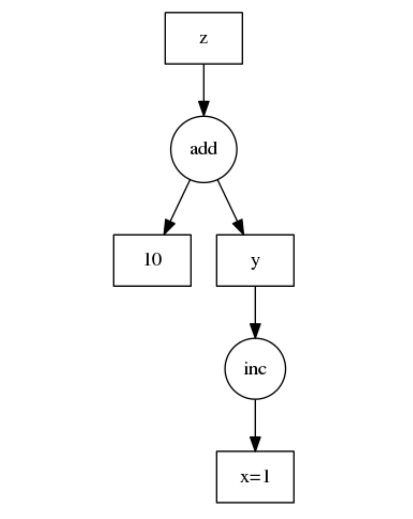
\includegraphics[scale=0.6]{images/grafo_dask.png}
	\caption[Ejemplo de grafo en dask.]{Ejemplo de grafo en dask. Fuente: \citep{rocklin2015dask}}
	\label{fig:dask_graph}
\end{figure}

\verb|Dask.array| es capaz de soportar la mayoría de las funcionalidades de Numpy como por ejemplo la operaciones aritméticas (+, - , *, exp, log, etc.), particionamiento, reducciones en los ejes (sum(), mean(), std()), álgebra lineal, indexación, entre otros. Sin embargo, no soporta algunas operaciones para arreglos con alguna dimensión con valor nulo, la mayoría de \verb|np.linalg| no está implementado, no implementa operaciones como \verb|tolist|, entre otros.

\newpage
